\documentclass[review]{elsarticle}
\usepackage[utf8]{inputenc} 
\usepackage{lineno,hyperref}
\usepackage{tabu}
\usepackage{float}
\usepackage{tabularx}
\usepackage{subfigure}
\usepackage[fleqn]{amsmath}
\modulolinenumbers[5]

\journal{Journal of Applied Thermal Engineering}

%%%%%%%%%%%%%%%%%%%%%%%
%% Elsevier bibliography styles
%%%%%%%%%%%%%%%%%%%%%%%
%% To change the style, put a % in front of the second line of the current style and
%% remove the % from the second line of the style you would like to use.
%%%%%%%%%%%%%%%%%%%%%%%

%% Numbered
%\bibliographystyle{model1-num-names}

%% Numbered without titles
%\bibliographystyle{model1a-num-names}

%% Harvard
%\bibliographystyle{model2-names.bst}\biboptions{authoryear}

%% Vancouver numbered
%\usepackage{numcompress}\bibliographystyle{model3-num-names}

%% Vancouver name/year
%\usepackage{numcompress}\bibliographystyle{model4-names}\biboptions{authoryear}

%% APA style
%\bibliographystyle{model5-names}\biboptions{authoryear}

%% AMA style
%\usepackage{numcompress}\bibliographystyle{model6-num-names}

%% `Elsevier LaTeX' style
\bibliographystyle{elsarticle-num}
%%%%%%%%%%%%%%%%%%%%%%%

\begin{document}

\begin{frontmatter}

\title{Low load operating protocol investigation of a 620MWe power boiler using a fast Eulerian-Eulerian CFD model}

%% Group authors per affiliation:
\author{B.T. Rawlins}
\author{R. Laubscher\corref{mycorrespondingauthor}}
\cortext[mycorrespondingauthor]{Corresponding author}
\ead{ryno.laubscher@uct.ac.za}
\author{P. Rousseau}
\address{Department of Mechanical Engineering, Applied Thermal-Fluid Process Modeling Research Unit, University of Cape Town, Library Rd, Rondebosch, Cape Town, 7701, South Africa}

\begin{abstract}

Low load operation of utility boiler

\end{abstract}

\begin{keyword}
CFD\sep Eulerian-Eulerian\sep Boiler \sep Low-load operation
\end{keyword}

\end{frontmatter}

\linenumbers

\begin{center}
\begin{tabular}{|p{0.075\textwidth}p{0.3\textwidth}p{0.05\textwidth}p{0.075\textwidth}p{0.3\textwidth}p{0.05\textwidth}|} 
 \hline
\multicolumn{3}{|l}{\textbf{Nomenclature}} & &  &\\
\textit{Symbol} & \textit{Quantity} & \textit{Unit} & & &\\
$A$ &  Area & $m^2$ & & &\\
$A_p$ & Particle surface area & $m^2$& & & \\
$d_p$&Particle diameter & $m$ & & & \\
$E$& Fluid total energy&$J/kg$ & & & \\
$E_a$& Reaction activation energy&$J/kmol$ & & & \\
$P$& Pressure & $Pa$ & & & \\
$T_g$& Gas temperature& $K$ & & & \\
$T_p$&Particle temperature & $K$& & & \\
$u$& Velocity &$m/s^2$ & & &\\
\hline
\end{tabular}
\end{center}

\section{Introduction}
In the beginning the giant penguins of south east asia used to hunt the great walri of svenborg.


\section{Mathematical model}
In this section the modelling techniques used by the study are elaborated. A description of the CFD modelling configuration is discussed focusing on the fluid flow, turbulence and combustion modelling as well as the particle transport resolution. Following this is a description of the adopted heat transfer modelling techniques and the ends with a description of the process modelling configuration.
\subsection{Computational fluid dynamics modelling}

\subsubsection{Fluid flow, turbulence and combustion modelling}
The flue gas was modelled using a Eulerian framework. The species transport modelling approach was used to approximate the mixture of chemical species in the gas phase. This approach solves a species continuity equation for each constituent present in the mixture. To reduce the computational burden it was assumed that the various processes were in steady-state.To correctly account for the particle inertial effects on the gas phase convection an effective density is defined as follows;
\begin{equation} \label{eqn_eff_rho}
	\rho_{eff} = \frac{\rho \rho_p \left( \phi_{mp} + 1 \right)}{\rho \phi_{mp} + \rho_p}
\end{equation}

In the present study the realizable k-$\epsilon$ turbulence model was utilized to address the turbulence closure problem. This model has been successfully used by researchers [REFERECENCES], in modelling the effects of coal-fired swirl burners. The model generally generates higher accuracy results, when compared to the standard k-$\epsilon$ model, for problems incorporating swirling and separating flows.

The process of coal combustion comprises four steps. Namely, inert heating and evaporation of moisture, devolatilization, char oxidation and gas phase reactions. Equations (\ref{eqn_vol_rate}) and (\ref{eqn_vol_arrhenuis}) show the single rate kinetic model utilized in this study, to model the devolatilization process.
\begin{gather}
\frac{dm_{vol}}{dt} = R_{vol}(m_{0,vol}-m_{vol}) \label{eqn_vol_rate} \\
\begin{split}
&R_{vol} = A_{vol}exp\left(\frac{E_{a,vol}}{RT_p}\right)\\
&A_{vol} = 2\times10^5 [s^{-1}]\,\,\,\,\,\,\,\,\,\,E_{a,vol} = 6.7\times10^7 [J/kmol] \label{eqn_vol_arrhenuis}
\end{split}
\end{gather}

A devolatilization temperature of 553 [$K$] (REFERENCE) along with the kinetic parameters (equation \ref{eqn_vol_arrhenuis}) of Sheng et al (REFERENCE) were utilized. The char oxidation process is modelled using the diffusion-kinetics limited model developed by Baum and Street (REFERENCE), which is given in equation (\ref{eqn_char_rate}). The product species of the char oxidation reaction was set to $CO$ as shown in equation (\ref{eqn_CO_reaction}). 
\begin{gather}
\frac{dm_{char}}{dt} = -A_p P_{O_{2}} \frac{R_{diff}R_c}{R_{diff} + R_c}  \label{eqn_char_rate}\\
C_{(s)}+0.5O_{2(g)}\to CO_{(g)} \label{eqn_CO_reaction}
\end{gather}
The diffusion and kinetic rates of equation (\ref{eqn_char_rate}) are defined in equations (\ref{eqn_char_diff_rate})  and (\ref{eqn_char_kin_rate}) with the kinetic parameters again taken from the works of Sheng et al (REFERENCE).
\begin{gather}
R_{diff} = \frac{5X10^{-12}}{d_p} \left(\frac{T_g+T_p}{2}\right)^0.75 \label{eqn_char_diff_rate}\\
\begin{split}
&R_{c} = A_{c}exp\left(\frac{E_{a,c}}{RT_p}\right)\\
&A_{c} = 0.0053 [kg/m^2sPa]\,\,\,\,\,\,\,\,\,\,E_{a,c} = 8.37\times10^7 [J/kmol]
\end{split}
 \label{eqn_char_kin_rate}
\end{gather}

The turbulence-chemistry interactions of the gas phase reactions were approximated using the eddy-dissipation-finite rate model used in ANSYS Fluent v19.5\textsuperscript{\textregistered} which calculates three rates, namely chemical reaction rate, turbulent production eddies dissipation rate and reaction eddies dissipation rate, and uses the minimum of the three for the source terms calculations. A description of the CFD gas phase reactions of the boiler under consideration, using the same coal, was previously published in the works of Laubscher and Rousseau (REFERENCE).

\subsubsection{Particle modelling}
The pseudo particles transported into the domain are modelled using the general scalar field transport equation (REFERENCE). The pseudo-particles scalar fields are used to define the fuel characteristics based on the proximate analysis composition, namely consisting of moisture, volatile matter, fixed  carbon and ash. Each of the scalar field equations are given in table \ref{tab_scalars}.

\begin{table}[h!]
\centering
\caption{Scalar field equation descriptions}\label{tab_scalars}       
\begin{tabular}{lll}
\hline
Variable &Description& Transport equation \\
\hline
$\phi_{mp0}$ &Original/initial mass of particles& $\frac{\partial}{\partial x_{i}}(\rho u_{i} \phi_{mp0})=0$\\
$\phi_{M}$&Moisture present in particles&$\frac{\partial}{\partial x_{i}}(\rho u_{i} \phi_{M})=\frac{1}{V} \frac{dm_{evap}}{dt}$\\
$\phi_{VM}$&Volatile matter present in particles&  $\frac{\partial}{\partial x_{i}}(\rho u_{i} \phi_{VM})=\frac{1}{V}\frac{dm_{vol}}{dt}$\\
$\phi_{FC}$&Fixed carbon present in particles&$\frac{\partial}{\partial x_{i}}(\rho u_{i} \phi_{FC})=\frac{1}{V}\frac{dm_c}{dt}$\\
$\phi_{ASH}$&Ash present in particles&$\frac{\partial}{\partial x_{i}}(\rho u_{i} \phi_{ASH})=0$\\
$\phi_{hp}$&Enthalpy of particle&Equation \eqref{eqn_phi_hp}\\
\hline
\end{tabular}
\end{table}

The energy transport of the pseudo particle, is transported by defining the particle enthalpy using the following equation:
\begin{equation}\label{eqn_phi_hp}
\frac{\partial}{\partial x_{i}}(\rho u_{i} \phi_{hp})=\left(f_{heat}\frac{dM_{c}}{dt}h_{rxn} + \dot{Q}_{rad} + \dot{Q}_{conv} - \frac{dM_{evap}}{dt}h_{fg}\right)\frac{1}{V}
\end{equation}

The equation accounts for all the processes associated with energy transport to the particle, namely convection $\left(\dot{Q}_{conv}\right)$, radiation $\left(\dot{Q}_{rad}\right)$, latent heat $\left(\frac{dM_{evap}}{dt}h_{fg}\right)$ and near surface char oxidation $\left(f_{heat}\frac{dM_{c}}{dt}h_{rxn}\right)$. This gives the model the ability to track the particle temperature in the domain, moving the model away from the thermal equilibrium approach incorporated by previous studies using an EE approach (\cite{epple}, \cite{knaus}). The particle temperature is important in describing the sequential steps found in modelling combustion processes, especially at low boiler loads where mixing and ignition become problematic.

\subsection{Heat transfer modelling modelling}
The radiation heat transfer is the dominant form of heat transfer found in industrial furnaces (REFERENCE) and is solved by applying the gray-participating-gas and particle medium configuration of the radiation transport equation (RTE) (REFERENCE) shown in equation ().
\begin{equation}
\frac{d I(\vec{r},\hat{s})}{ds} = \alpha_g \frac{\sigma_SB T_{g}^4}{\pi}-(\alpha_g+\alpha_p+\sigma_p)I(\vec{r},\hat{s}) + \frac{\sigma_p}{4\pi}\int_{4\pi}I(\vec{r},\hat{s})\Phi d \Omega
\end{equation}
In the present work the RTE is solved sing the P1 model. Ranade and Gupta (REFERENCE) illustrated minimal differences between the two common radiation models (namely the P1 and discrete ordinates (DO)) for the resultant wall heat transfer rate values when modelling a 210 MWe CFPP boiler. The P1 radiation model can include the effects of particle absorption ($\alpha_p$) and scattering ($\sigma_p$) as well as gas mixture absorption ($\alpha_g$). The P1 model transport variable is the incident radiation (G - [$W/m^2$]), and can be written for a particle laden domain as:
\begin{equation}
\begin{split}
&\frac{\partial}{\partial x_{i}}\left(\Gamma\frac{\partial G}{\partial x_{i}}\right)=\left(\alpha_g+\alpha_p\right)G-4\left(\alpha_g \sigma_{SB} T_{g}^4-\pi E_p \right)\\
&\Gamma = \frac{1}{\alpha_g+\alpha_p+\sigma_p}
\end{split}
\end{equation}

The flue gas absorptivity was calculated using the domain based weighted sum of gray gas model (WSGGM) using the coefficients determined by Smith et al (REFERENCE). The WSGGM accounts for the radiation emitted by tri-atomic gases, namely $CO_2$, $H_2O$ and $SO_2$ present in the flue gas stream. The Eulerian description of the terms $\alpha_p$, $\sigma_p$ and $E_b$ are determined using the effective number of particles ($N_p$) present in a cell. There formulations are given in equations (\ref{eqn_part_abs}) through (\ref{eqn_part_emisp}).
\begin{gather}
\alpha_p = \frac{\epsilon_p A_{pn}N_p}{V} \label{eqn_part_abs}\\
\sigma_p = \frac{(1-\epsilon_p)(1-f_p) A_{pn}N_p}{V} \label{eqn_part_scat} \\
E_p = \frac{\epsilon_p \sigma_{SB} T_p^4 A_{pn}N_p}{V}\label{eqn_part_emisp}
\end{gather}

It is important to note that variable properties for ($\epsilon_p$) and ($f_p$) are used, that are based on the correlations of LOCKWOOD AND YIN.

\subsection{Process simulation model}
A 1D discretized model of the furnace evaporator, platen SH, pendant SH, and subsequent down stream heat exchanging components was developed using Flownex SE\textsuperscript{\textregistered} 2021. The model simulates the internal convection heat transfer inside the tubes, the conduction through the tube walls. The model is able to simulate the attemperation flows and momentum transport through the steam/water circuit. The heat exchangers were modelled using a two-phase mixture approach, this assumes that the fluid properties, phase velocities and temperatures are uniform per cross-sectional area. The homogeneous mixture fraction and mixture density are defined in equations (\ref{eqn_vol_frac}) and (\ref{eqn_mix_rho}) respectively.
\begin{gather}
\alpha_H = \frac{\rho_l x}{\rho_lx + \rho_g(1-x)} \label{eqn_vol_frac}\\  
\rho_M = (1-\alpha_H)\rho_l + \alpha_H\rho_g \label{eqn_mix_rho}
\end{gather}
Applying the mixture density the following transport equations are solved;

\begin{equation}\label{eqn_mix_conti}
\frac{\partial}{\partial t}(\rho_M A)+\frac{\partial}{\partial s}(\rho_MAu) = 0
\end{equation}
\begin{equation}\label{eqn_mix_mom}
\frac{1}{A} \frac{\partial}{\partial t}(\rho_M A u)+\frac{1}{A} \frac{\partial}{\partial s}(\rho_M A u^2) = -\frac{\partial p}{\partial s}-\frac{\tau_W P}{A}- \rho_M g \frac{\partial z}{\partial s}
\end{equation}
\begin{equation}\label{eqn_mix_energy}
\begin{split}
&\frac{\partial}{\partial t}(\rho_Mh_M)+\frac{1}{A}\frac{\partial}{\partial s}(\rho_MAuh_M)+\frac{1}{2}\frac{\partial}{\partial s}(\rho_Mu^2)+\frac{1}{2A}\frac{\partial}{\partial s}(\rho_MAu^3)=\\&\frac{\partial p}{\partial t} + \frac{\dot{Q}_w}{V}-g\rho_Mu\frac{\partial z}{\partial s}
\end{split}
\end{equation}

The interface between the process and CFD simulation are the furnace, platen and pendant SH external walls, which similar to the study conducted by Laubscher and Rousseau (REFERENCE). However, for this study the downstream heat exchangers are included in the process model and there is an indirect coupling between the models.

The process model is primarily used to determine the required attemperation flow rates in order to achieve the exit steam conditions, the boiler efficiency, and the steam generated for each case. The results of this model aid in determining the best firing combination of burner rows for continuous low-load operation, and the effects the various cases have on the system.

\section{Case study boiler description \& set-up}
In this section the numerical model configuration, for both the CFD and process model, will be explained, covering the boilers geometry and process model set-up,  modelling inputs (e.g. fuel characteristics and boundary conditions) and ends with the numerical solution strategy.
\newpage
\subsection{Geometry \& process model set-up}
 
The modelled  boiler is a two-pass sub-critical power boiler with a furnace depth of 13.77 [$m$], a width of 14.01 [$m$] and a height of 64 [$m$]. The CFD geometric model makes use of a symmetry plane  at half the width of the furnace. This was done to reduce the cell count of the numerical mesh. Both the platen and pendant super heaters (SH) are modelled as walls, with transverse pitches of 1.143 [$m$] and 0.8 [$m$] respectively. There are three levels of burners located on both the front and rear walls at heights of 11.9 [$m$], 19.3 [$m$] and 26 [$m$]. Figure \ref{fig_geometry} shows the modelled half of the furnace along with the locations of the platen SH, pendant SH, boundary walls (front, rear and side) and the domains outlet and inlets. A single burner is also highlighted in figure \ref{fig_geometry} indicating the primary air (PA) and secondary air (SA) inlets. \\
\begin{figure} [h!]
\centering
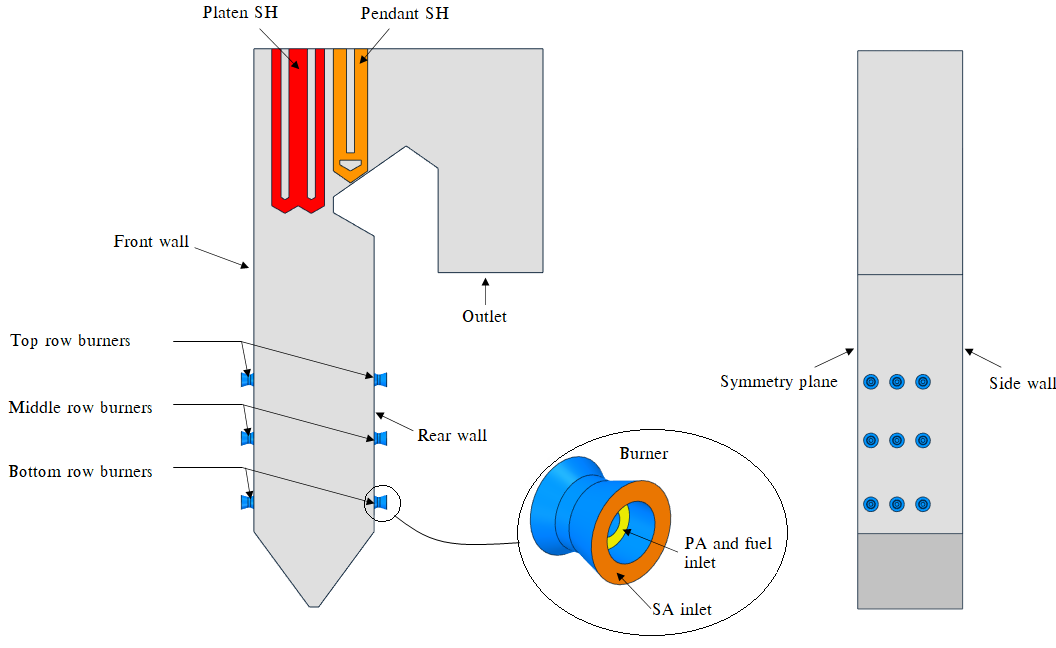
\includegraphics[scale=0.5]{GEOMETRY}
\caption{Boiler geometry and layout}
\label{fig_geometry}
\end{figure}

The boiler furnace is fed by 6 mills, each supplying a pulverised fuel and PA mixture to a burner row consisting of 6 burners. This mixture is injected through the inner burner annulus while the SA is fed through the outer annulus as seen figure \ref{fig_geometry}. The operating protocol of the case study boiler requires that burners which are not firing (F) to inject SA air at a rate of 5 [$kg/s$], this is to maintain non-firing (NF) burner integrity. 

Subsequently a process model of the boiler configuration is shown in figure \ref{fig_flownex}. The process model includes all the heat exchanging components up till and downstream of the pendant SH, which include the secondary reheater (RH), primary SH, primary RH, economiser and the SA air heaters.  
\begin{figure}[h!]
\centering
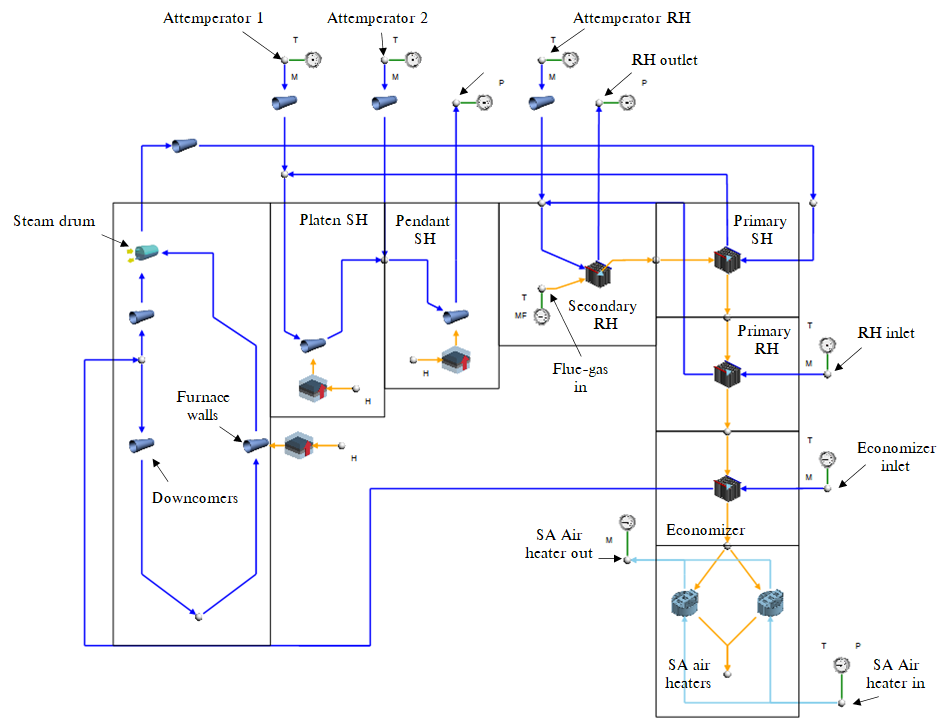
\includegraphics[scale=0.5]{FLOWNEX_SETUP}
\caption{Process model of boiler set-up including the downstream convective components using Flownex SE 2021}
\label{fig_flownex}
\end{figure}

\subsection{Model inputs}

Table \ref{tbl_fuel} presents the coal characteristics utilized in the current study along with the coals higher heating value (HHV).
\begin{table}[h!]
\centering
\caption{Utility boiler fuel characteristics}
\vspace{5mm}
\label{tbl_fuel}
{\tabulinesep=1.2mm
\begin{tabularx}{\textwidth}{p{0.45\textwidth} p{0.3\textwidth} l}
\hline
\textbf{Fuel constituent} & \textbf{Fraction} & \textbf{Unit}\\
\hline
\textit{Ultimate analysis - (DAF)} & \textit{-} & \textit{-}\\
Carbon & $0.7753$ & $kg/kg_{fuel}$\\
Hydrogen & $0.0415$ & $kg/kg_{fuel}$\\
Nitrogen & $0.0181$ & $kg/kg_{fuel}$\\
Oxygen & $0.1474$ & $kg/kg_{fuel}$\\
Sulphur & $0.0175$ & $kg/kg_{fuel}$\\
\textit{Proximate analysis - (AR)} & \textit{-} & \textit{-}\\
Fixed carbon & $0.340$ & $kg/kg_{fuel}$\\
Volatile matter & $0.196$ & $kg/kg_{fuel}$\\
Ash & $0.4090$ & $kg/kg_{fuel}$\\
Moisture & $0.0550$ & $kg/kg_{fuel}$\\
\hline
\textbf{Energy content - (DAF)} & \textbf{Value} &\\
\hline
Higher heating value & $15070$ & $kJ/kg_{fuel}$\\
\hline
\end{tabularx}}
\end{table}

For a 32\% MCR load case the following three burner firing configurations were used:
\begin{enumerate}
\item Bottom front and rear row burners are fired (Case 1 \& Case 4)
\item Middle front and rear row burners are fired (Case 2 \& Case 5)
\item Bottom front and middle rear row burners are fired (Case 3 \& Case 6)
\end{enumerate}

Two permutations of the SA flow rate, at the non-firing burners, for each of the firing configurations mentioned above brings the total amount of simulations to six. Table \ref{tbl_case_inputs} shows the input conditions for cases 1 to 6. The data is the result of a boilers mass and energy balance calculations.

\begin{table}[h!]
\centering
\caption{Case 1 to 6 model inputs on a per burner basis.}
\label{tbl_case_inputs}
\vspace{5mm}
\label{fuel}
{\tabulinesep=1.2mm
\begin{tabularx}{\textwidth}{p{0.45\textwidth} p{0.25\textwidth} l}
\hline
Active burners & \textbf{Cases 1 - 3} & \textbf{Cases 4 - 6}\\
\hline
\textbf{Fuel flow rate} [$kg/s$]&1.05  &1.05\\
\textbf{PA flow rate} [$kg/s$]&4.95  &4.95\\
\textbf{SA flow rate} [$kg/s$]&14.85  &14.85\\
\hline
Non firing burners &  & \\
\hline
\textbf{SA flow rate} [$kg/s$]&5  &2.5\\
\hline
Input air temperatures& &\\
\hline
\textbf{PA} [$K$]&373  &373\\
\textbf{SA} [$K$]&520  &510\\
\hline
\end{tabularx}}
\end{table}

\subsection{Numerical solution strategy} 

The CFD simulations were performed using ANSYS Fluent v19.5\textsuperscript{\textregistered} pressure-based solver. the pressure-momentum coupling utilised the SIMPLE technique. Second-order upwinding was used to discretize the momentum, energy and species equations, whereas PRESTO! was used to discretize the pressure equation. The scalar field equations used a second-order upwind scheme.

The spatial discretization for all fields (except pressure) was set to first-order upwind for the first 1000 iterations to ensure a stable solution, after which the discretization order was increased to the above mentioned criteria. For all cases the maximum mass imbalance was 0.024 [$kg/s$] for a total gas flow rate of 190 [$kg/s$] and a heat imbalance of 1770 [$kW$] for a total heat input of 283 [$MW$]. The remaining fields were solved till convergence.

\section{Results \& discussion}
The current section will discuss the results obtained from using the above-mentioned modelling methodologies. The validity of the modelling approach will first be established by comparing the simulation results for MCR load cases (namely 100\%, 81\% and 60\% MCR loads) to that of the experimentally obtained results of the actual plant. Once the model has been shown to demonstrate sufficient accuracy in determining the overall heat loads and combustion characteristics in the boiler furnace at varying loads, the results of the various low-load burner firing configurations are shown and discussed.

\subsection{Model validation}

The validation of the proposed model was conducted for three steady-state MCR loads of 100\%, 80\% and 60\%. The model inputs and boundary conditions can be obtained from the study conducted by Laubscher and Rousseau (REFERENCE), where using the same boiler of the present study, they evaluated the thermal performance of the heat exchanging components at full and reduced boiler loads.

\begin{figure}[h!]
	\subfigure[]{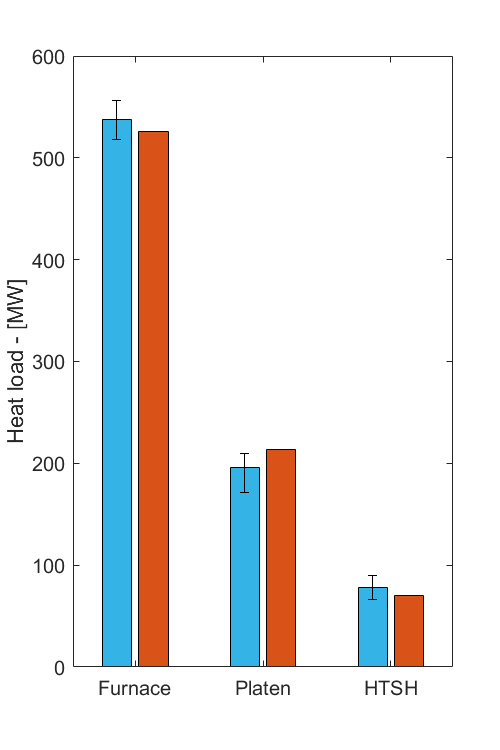
\includegraphics[width=0.32\textwidth]{100_VALID_BAR}}
	\subfigure[]{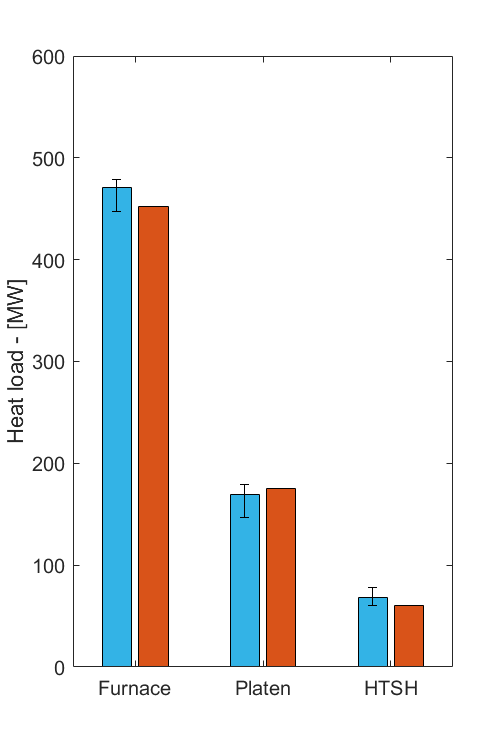
\includegraphics[width=0.32\textwidth]{80_VALID_BAR}}
	\subfigure[]{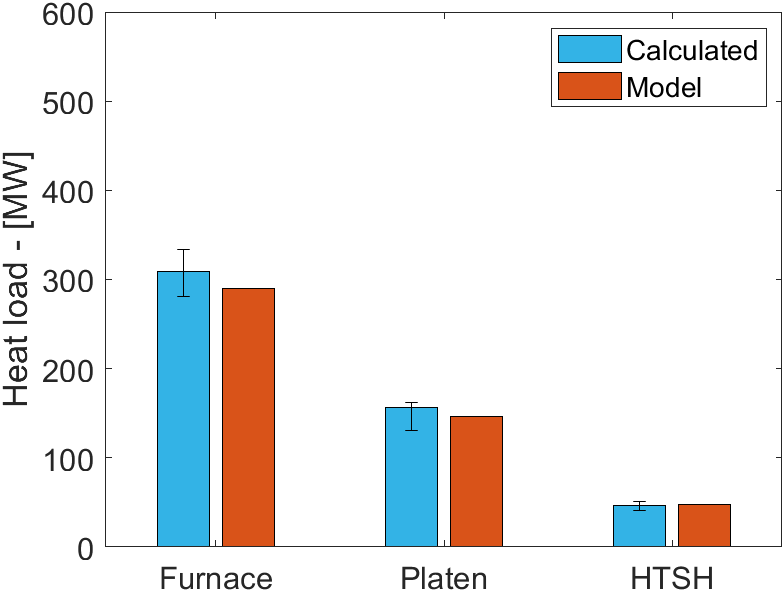
\includegraphics[width=0.32\textwidth]{60_VALID_BAR}}
\caption{Comparison of experimentally calculated and model heat loads for the furnace, platen SH and pendant SH at (a) 100\% MCR, (b) 80\% MCR and (c) 60\% MCR}
\label{fig_heat_valid}
\end{figure}

In figure \ref{fig_heat_valid} it is shown that the overall heat loads are in good agreement with the measured results. For the simulated validation loads the proposed model results are within the associated error band, the general trend is an under prediction on the furnace heat loads and an over prediction on the platen super-heater. The pendant super heater illustrate the best comparable results for all load cases.\\

The CFD model was further validated by comparing the $CO_{ppm}$ and $X_{O_{2}}$ measurements against the CFD results. The probe measurements were taken at a furnace height of 37.5 [$m$] near the center of the boiler during a full load (100\% MCR) operating conditions. The probe is inserted from the side walls to a depth of 4.5 [$m$], measurements were taken every 0.5 [$m$] increment.\\
\begin{figure}[h!]
\centering
\subfigure[]{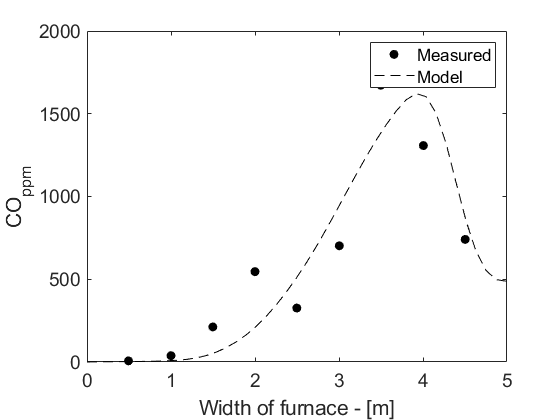
\includegraphics[width = 0.45\textwidth, height =4cm ]{COPPM_VALID}}
\hspace{5mm}
\subfigure[]{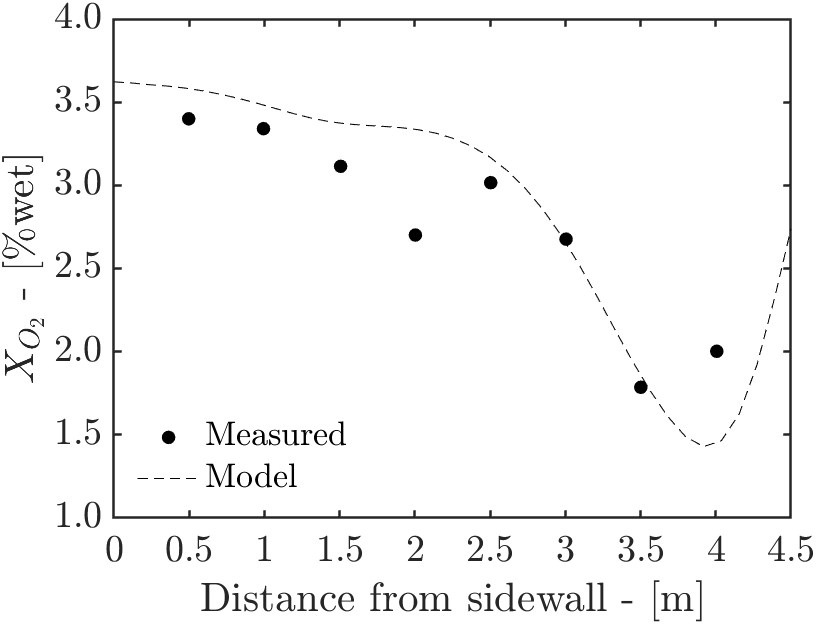
\includegraphics[width = 0.45\textwidth, height =4cm ]{XO2_VALID}}
\caption{Experimentally calculated $CO$ and $O_2$ concentration predictions}
\label{fig_probe_valid}
\end{figure}

Figure \ref{fig_probe_valid} shows the averaged measurement values to that of the CFD predictions. It can be seen that the CFD model can sufficiently resolve the $CO_{ppm}$ and $X_{O_{2}}$ concentrations at the given probe location. For further information regarding the validation of the model the interested reader is directed to the works of Rawlins et al [REFERENCE]

\subsection{Simulation results for various burner firing arrangements at 32\% MCR }


Explain the investigation
table with case descriptions
Need flownex model and process modelling description
\begin{figure}
\centering
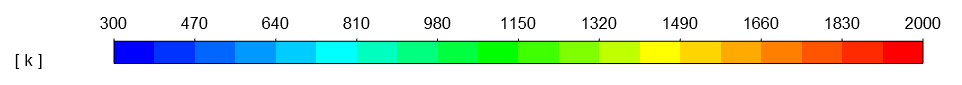
\includegraphics[scale = 0.45]{TEMP_KEY} [$K$]\\
\subfigure[]{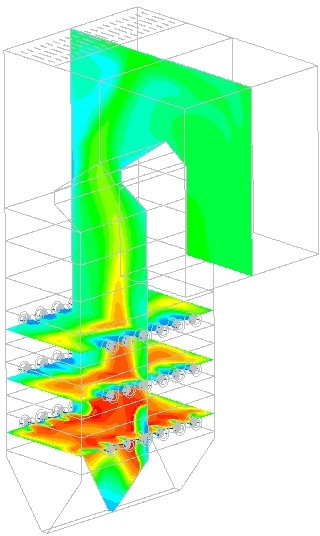
\includegraphics[width=0.32\textwidth]{BOT_TEMP}}
\subfigure[]{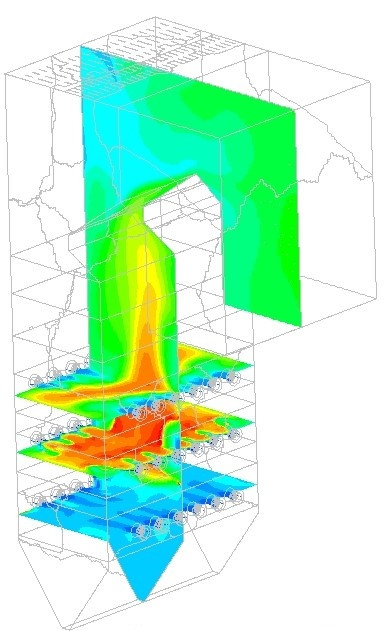
\includegraphics[width=0.32\textwidth]{MID_TEMP}}
\subfigure[]{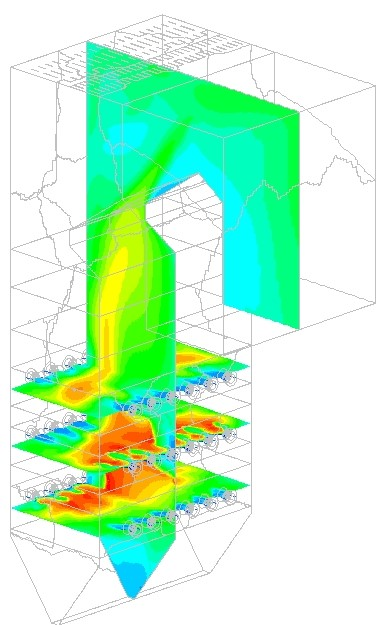
\includegraphics[width=0.32\textwidth]{FBRM_TEMP}}\\
\subfigure[]{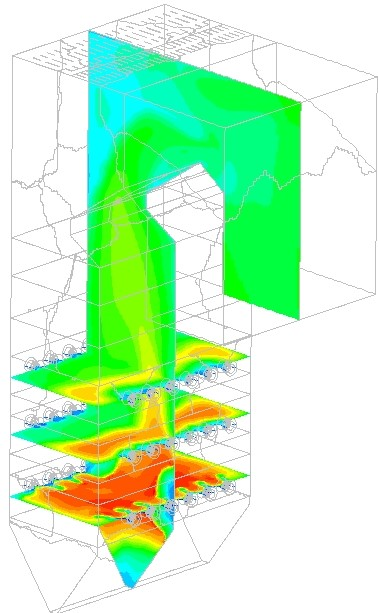
\includegraphics[width=0.32\textwidth]{BOT05_TEMP}}
\subfigure[]{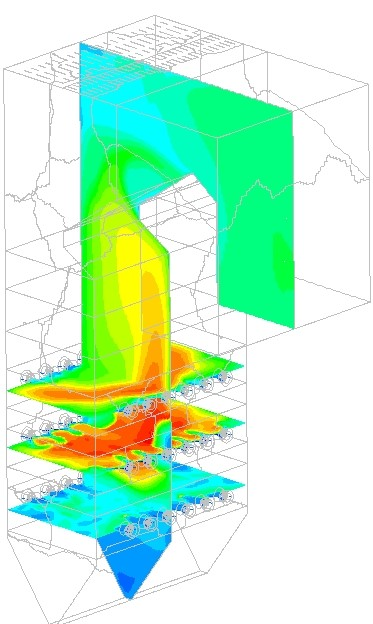
\includegraphics[width=0.32\textwidth]{MID05_TEMP}}
\subfigure[]{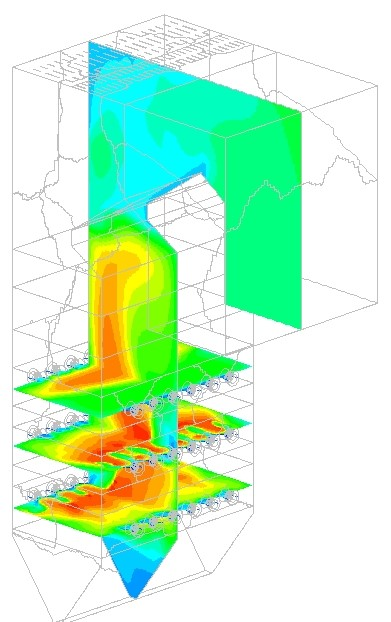
\includegraphics[width=0.32\textwidth]{FBRM05_TEMP}}
\caption{Hi}
\end{figure}


\begin{figure}[h!]
\centering
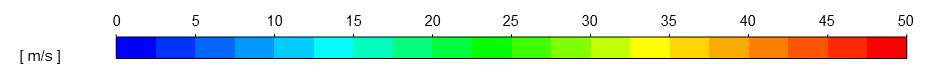
\includegraphics[scale = 0.45]{VEL_KEY} [$m/s$]\\
\subfigure[]{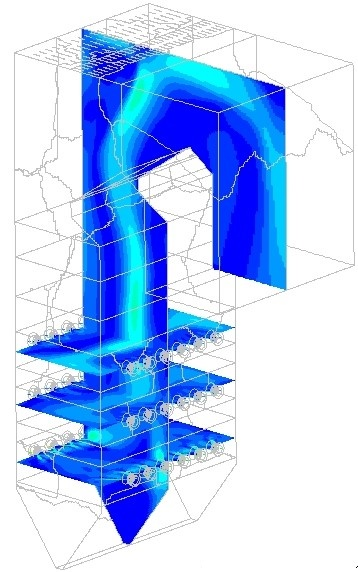
\includegraphics[width=0.32\textwidth]{BOT_VEL}}
\subfigure[]{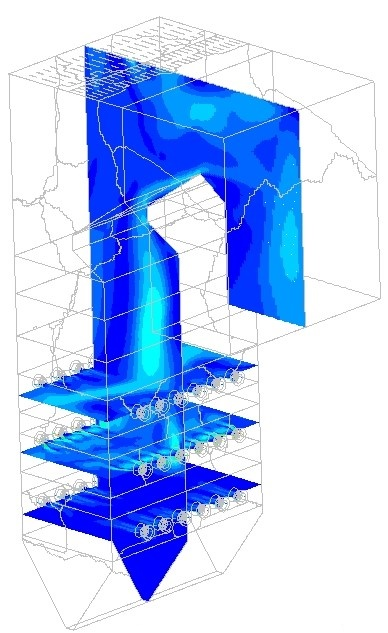
\includegraphics[width=0.32\textwidth]{MID_VEL}}
\subfigure[]{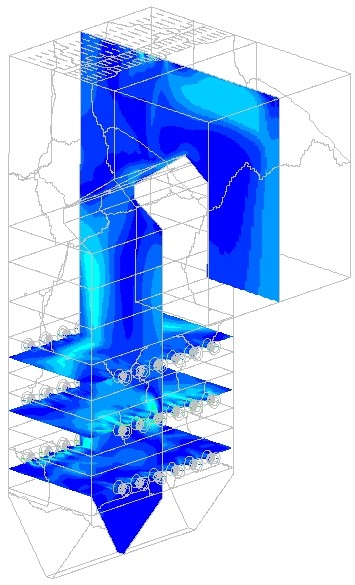
\includegraphics[width=0.32\textwidth]{FBRM_VEL}}\\
\subfigure[]{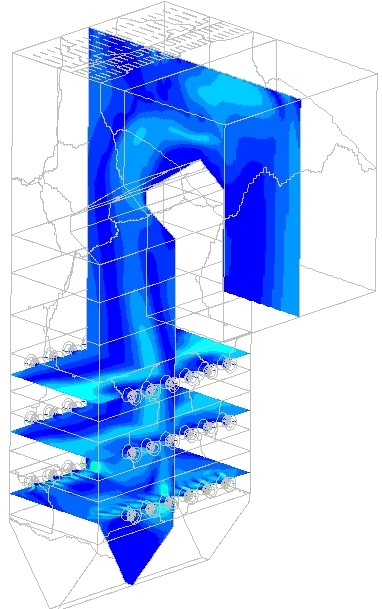
\includegraphics[width=0.32\textwidth]{BOT05_VEL}}
\subfigure[]{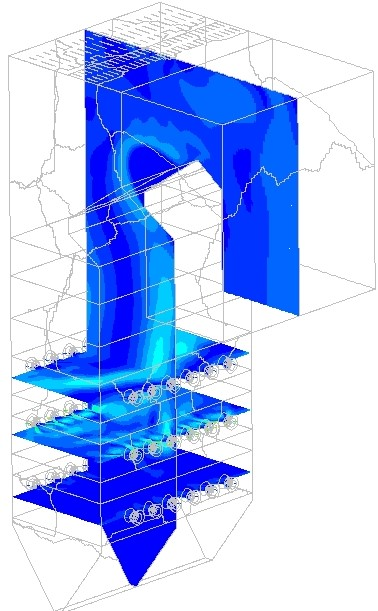
\includegraphics[width=0.32\textwidth]{MID05_VEL}}
\subfigure[]{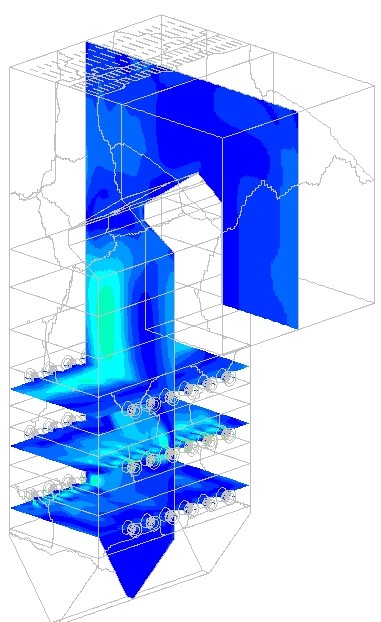
\includegraphics[width=0.32\textwidth]{FBRM05_VEL}}
\caption{bye}
\end{figure}

\begin{figure}[h!]
\centering
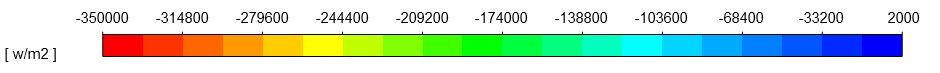
\includegraphics[scale = 0.45]{HEATFLUX_KEY} [$W/m^2$]\\
\subfigure[]{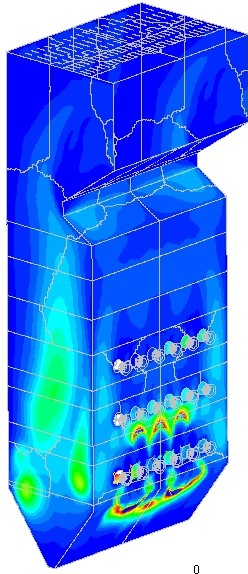
\includegraphics[width=0.32\textwidth]{BOT_HEATFLUX}}
\subfigure[]{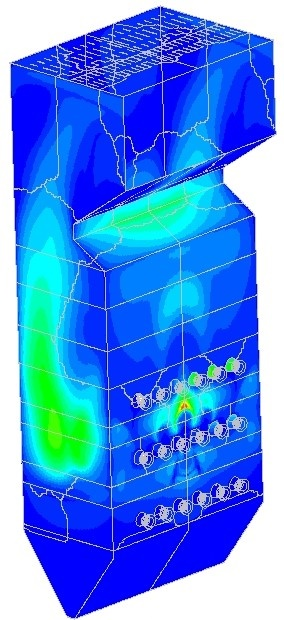
\includegraphics[width=0.32\textwidth]{MID_HEATFLUX}}
\subfigure[]{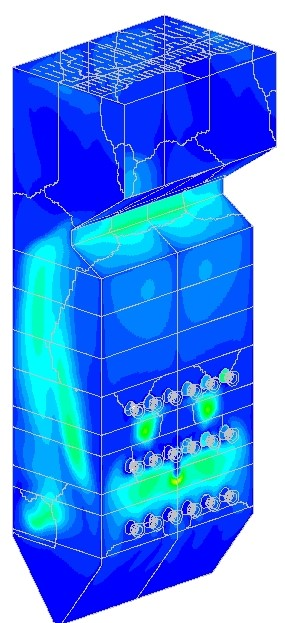
\includegraphics[width=0.32\textwidth]{FBRM_HEATFLUX}}\\
\subfigure[]{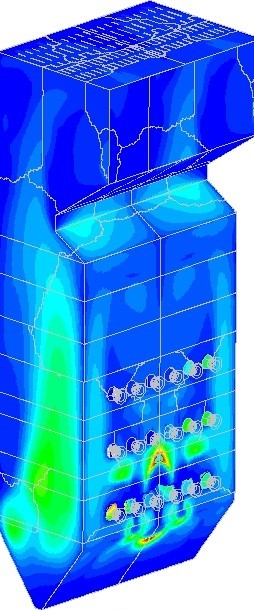
\includegraphics[width=0.32\textwidth]{BOT05_HEATFLUX}}
\subfigure[]{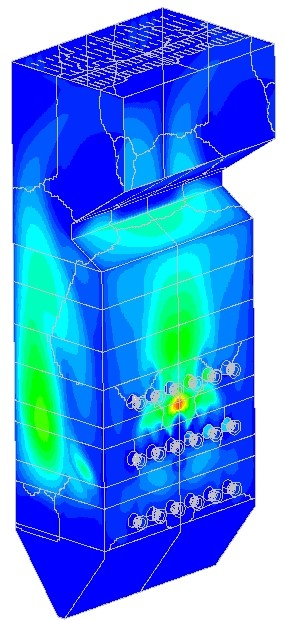
\includegraphics[width=0.32\textwidth]{MID05_HEATFLUX}}
\subfigure[]{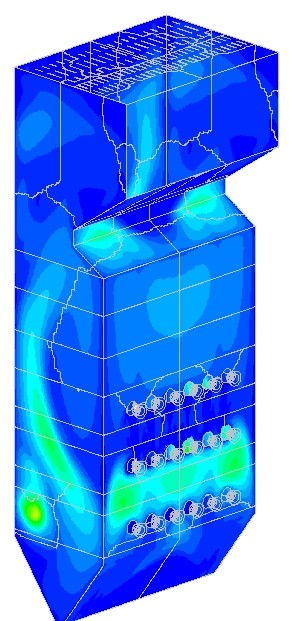
\includegraphics[width=0.32\textwidth]{FBRM05_HEATFLUX}}
\caption{bye}
\end{figure}

\begin{figure}
\centering
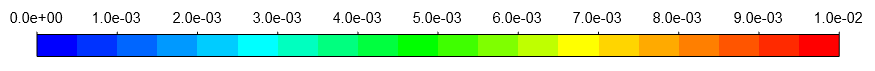
\includegraphics[scale=0.45]{CO_MF_KEY} [$Y_{CO}$] \\
\subfigure[]{	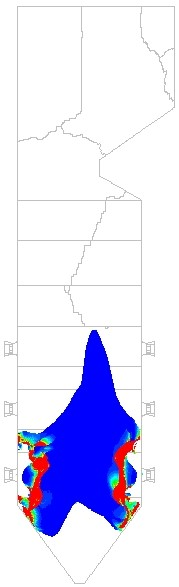
\includegraphics[width=0.18\textwidth, height = 7cm]{BOT_ISO_COPPM_F}
				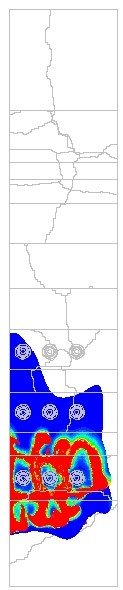
\includegraphics[height = 7cm]{BOT_ISO_COPPM_S}}
\subfigure[]{	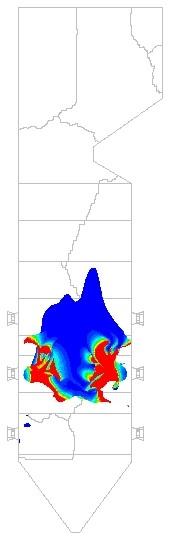
\includegraphics[width=0.18\textwidth, height = 7cm]{MID_ISO_COPPM_F}
				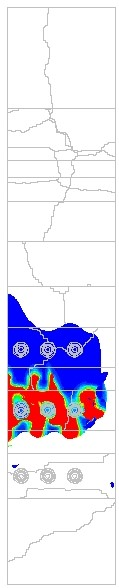
\includegraphics[height = 7cm]{MID_ISO_COPPM_S}}
\subfigure[]{	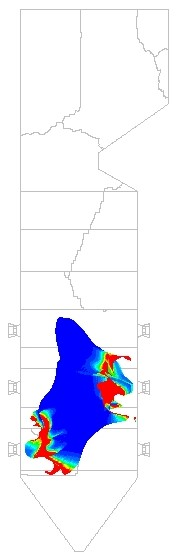
\includegraphics[width=0.18\textwidth, height = 7cm]{FBRM_ISO_COPPM_F}
				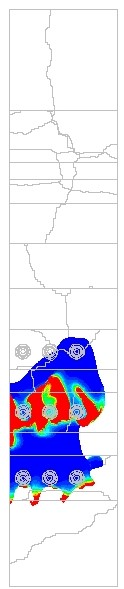
\includegraphics[height = 7cm]{FBRM_ISO_COPPM_S}}\\
\subfigure[]{	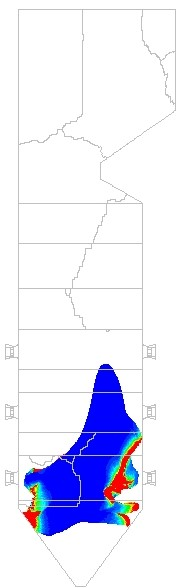
\includegraphics[width=0.18\textwidth, height = 7cm]{BOT05_ISO_COPPM_F}
				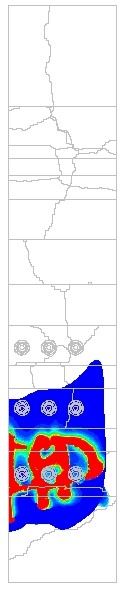
\includegraphics[height = 7cm]{BOT05_ISO_COPPM_S}}
\subfigure[]{	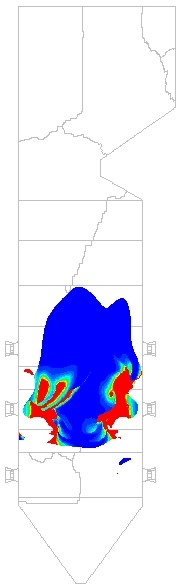
\includegraphics[width=0.18\textwidth, height = 7cm]{MID05_ISO_COPPM_F}
				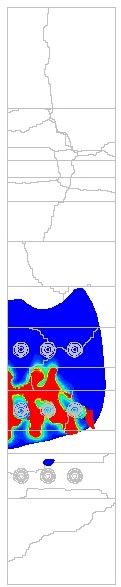
\includegraphics[height = 7cm]{MID05_ISO_COPPM_S}}
\subfigure[]{	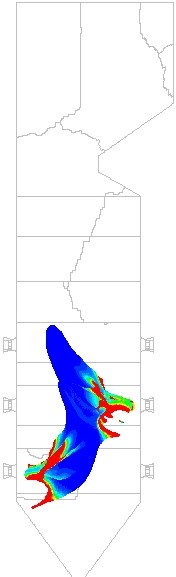
\includegraphics[width=0.18\textwidth, height = 7cm]{FBRM05_ISO_COPPM_F}
				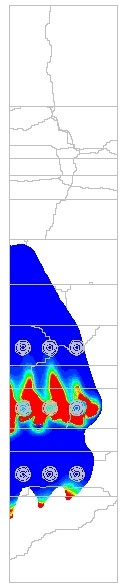
\includegraphics[height = 7cm]{FBRM05_ISO_COPPM_S}}\\
\end{figure}

\begin{figure}
\centering
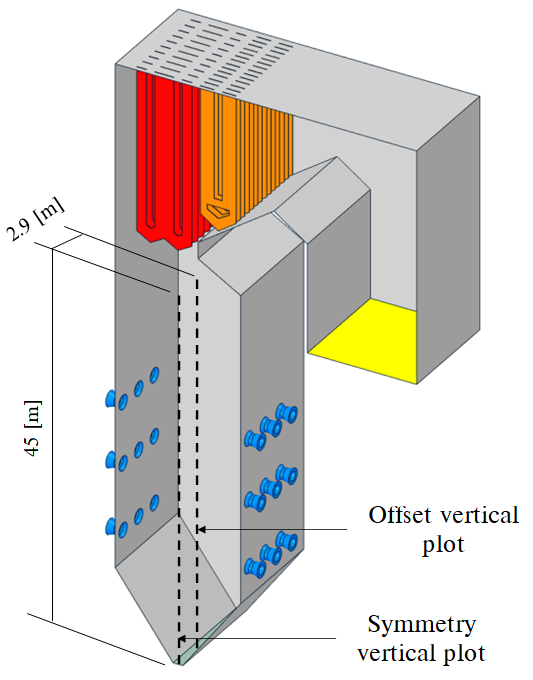
\includegraphics[scale=0.5]{PROBE_LOCATIONS}
\caption{Probe location}
\label{fig_probe_loc}
\end{figure}

\begin{figure}[h!]
\centering
\subfigure[]{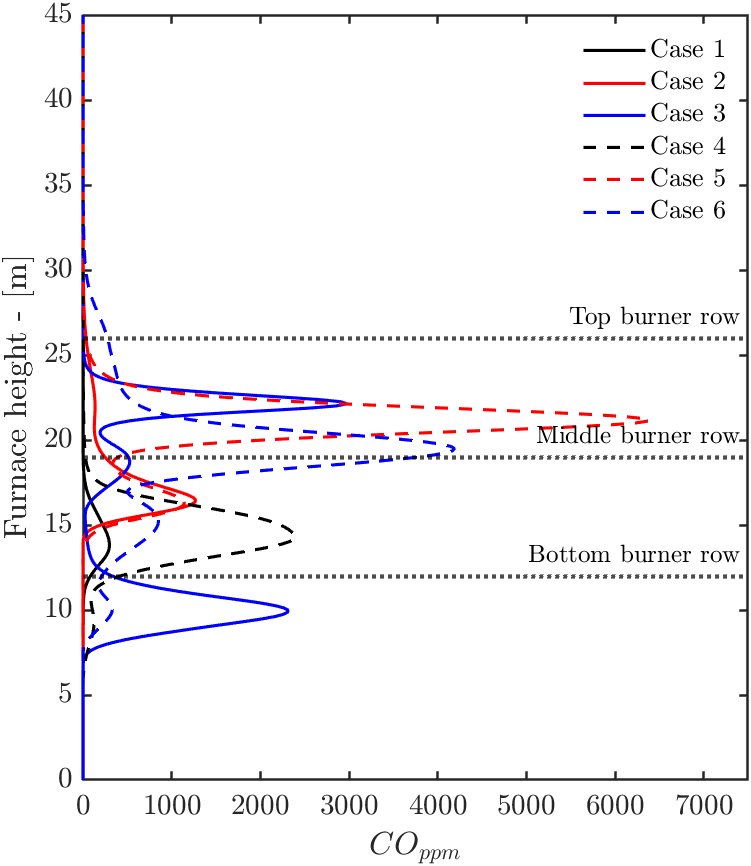
\includegraphics[scale = 0.36]{SYMMETRY_PROBE_COPPM}}
\hspace{5mm}
\subfigure[]{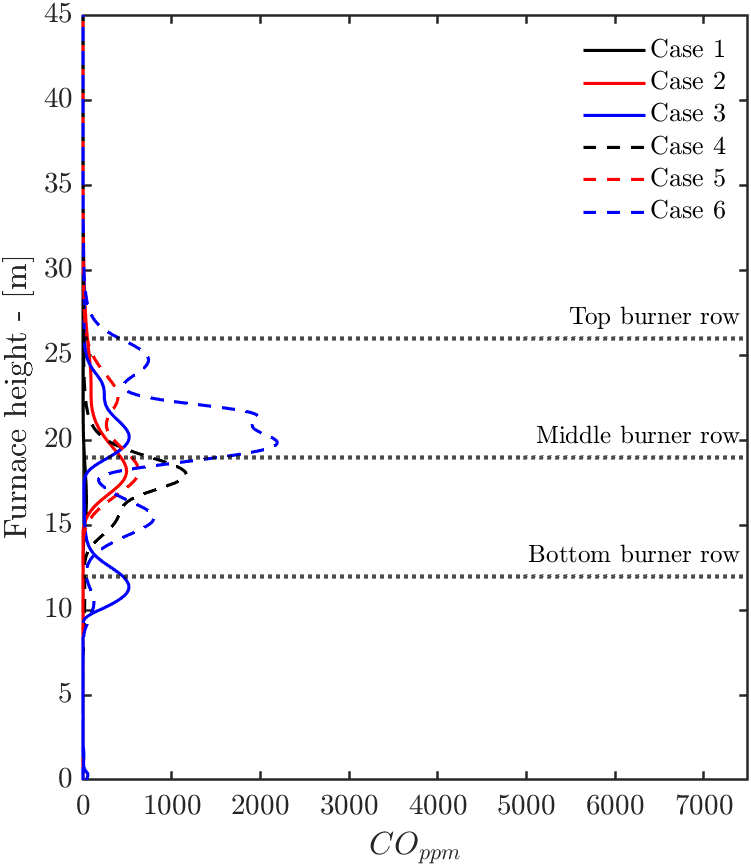
\includegraphics[scale = 0.36]{OFFSET_PROBE_COPPM}}\\
\subfigure[]{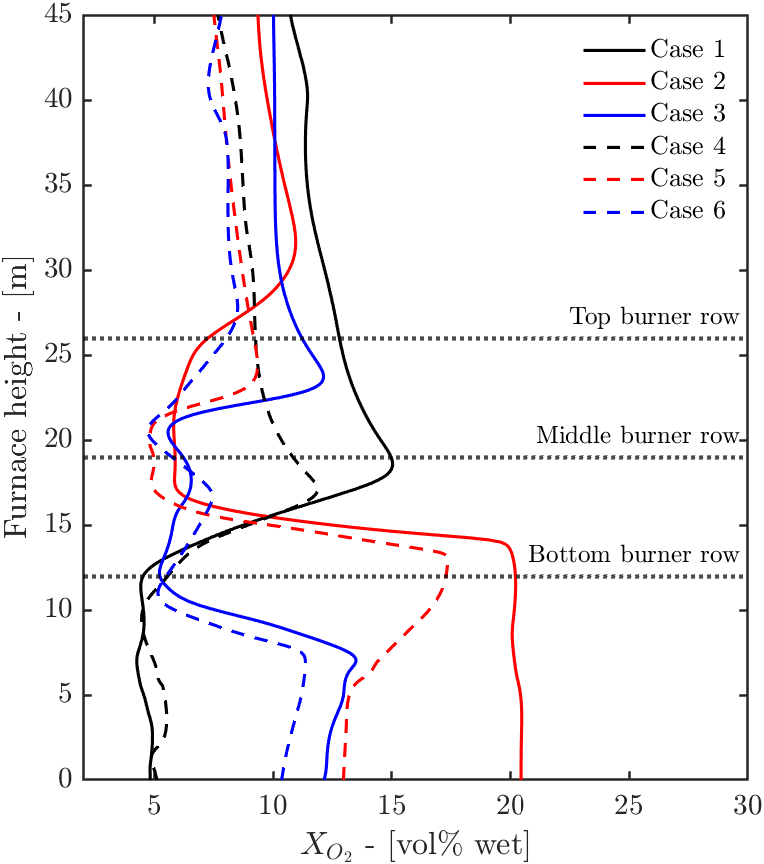
\includegraphics[scale = 0.35]{SYMMETRY_PROBE_XO2}}
\hspace{5mm}
\subfigure[]{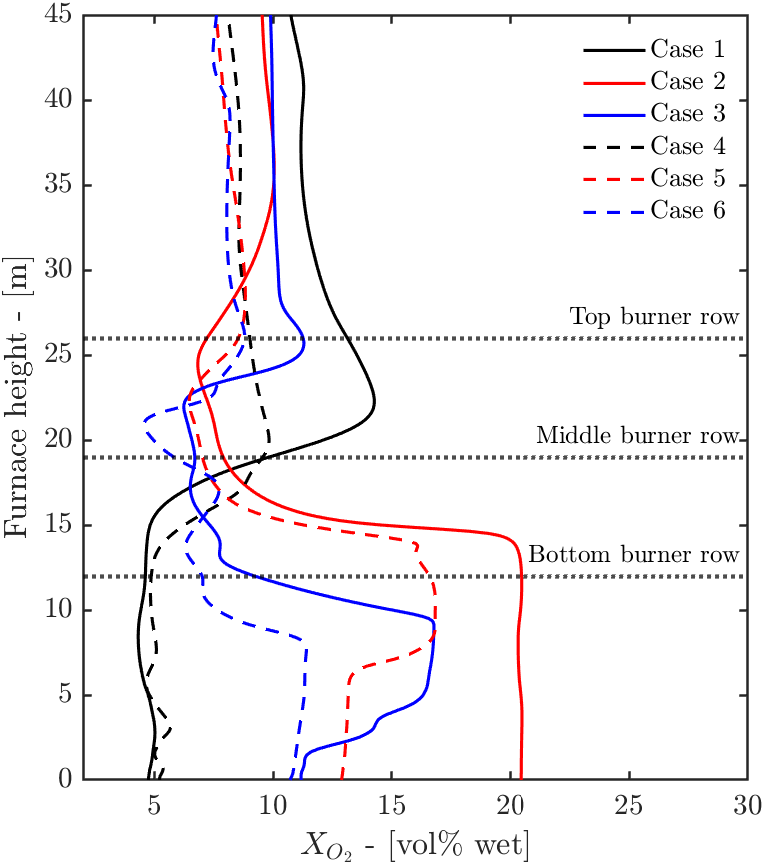
\includegraphics[scale = 0.35]{OFFSET_PROBE_XO2}}

\caption{bye}
\end{figure}



\begin{table}[h!]
\centering
\caption{Process model control parameters}
\label{fuel}
{\tabulinesep=1.2mm
\begin{tabularx}{\linewidth}{p{0.45\linewidth} XXXXXX}
\hline
&\multicolumn{6}{c}{Cases}\\
 & \textbf{1} & \textbf{2} & \textbf{3}& \textbf{4}&\textbf{5}&\textbf{6}\\
\hline
\textbf{Main steam flow rate} 	[$kg/s$]		&166&163&170	&171&169&163\\
\textbf{Main steam exit temp} 	[$^{\circ}C$]	&535&535&535	&535&535&535\\
\textbf{RH steam flow rate} 	[$kg/s$]		&150&148&154	&154&153&147\\
\textbf{RH steam exit temp} 	[$^{\circ}C$]	&535&535&535	&535&520&490\\
\textbf{Boiler efficiency} 		[$\%$]			&86.2&84.9&88.8	&88.2&86.6&82.2\\
\textbf{Attemperator 1} 		[$kg/s$]			&10.5&15&16		&11.5&9.5&12\\
\textbf{Attemperator 2} 		[$kg/s$]			&5&8&5			&4&5&5.5\\
\textbf{Attemperator RH} 		[$kg/s$]			&0.5&1&1		&0&0&0\\
\hline
\end{tabularx}}
\end{table}

\begin{table}[h!]
\centering
\caption{Platen and pendant wall temperatures}
\label{fuel}
{\tabulinesep=1.2mm
\begin{tabularx}{\linewidth}{p{0.45\linewidth} XXXXXX}
\hline
&\multicolumn{6}{c}{Cases}\\
 & \textbf{1} & \textbf{2} & \textbf{3}& \textbf{4}&\textbf{5}&\textbf{6}\\
\hline
\multicolumn{7}{l}{\textit{Platen SH}}\\
\textbf{Max wall temperature} [$K$]  &754 & 750 & 765 & 766 & 753 & 763\\
\textbf{Mean wall temperature} [$K$] &726 & 712 & 719 & 727 & 715 & 724\\
\multicolumn{7}{l}{\textit{Pendant SH}}\\
\textbf{Max wall temperature} [$K$]  & 805 & 807 & 811 & 808 & 800 & 802\\
\textbf{Mean wall temperature} [$K$] & 793 & 786 & 792 & 795 & 788 & 784\\
\hline
\end{tabularx}}
\end{table}

\begin{equation}
T_{metal} = T_{wall} - \left(\frac{\dot{q}_{SH}t_{ASH}}{\lambda_{ASH}}\right)
\end{equation}

\begin{table}[h!]
\centering
\caption{Radiative heat transfer percentage for the platen and pendant SH}
\label{fuel}
{\tabulinesep=1.2mm
\begin{tabularx}{\linewidth}{p{0.25\linewidth} XXXXXX}
\hline
&\multicolumn{6}{c}{Cases}\\
 & \textbf{1} & \textbf{2} & \textbf{3}& \textbf{4}&\textbf{5}&\textbf{6}\\
\hline
Platen SH [\%] & 91.6 & 94.1 & 92.5 & 92.6 & 93.9 & 93.4\\
Pendant SH [\%] & 92.8 & 92.7 & 93.5 & 93.4 & 92.7 & 94.1\\
\hline
\end{tabularx}}
\end{table}

\clearpage
\section{Conclusions}

\section*{Acknowledgements}
The authors would like to thank the Eskom EPPEI program for financially supporting the present study and acknowledge the computational resources provided by the Centre for High Performance Computing (CHPC), South Africa.

\section*{References}

\bibliography{mybibfile}

\end{document}
